%
% Barren Planet - User Manual
% Main document source
%
% Copyright (C) Damian Gareth Walker 2022
% Manual Sections: Starting Off
%
% Structure:
% Introductory
% Controls
% - Settings window
% - Menu
% Choosing a side
% - Choice of sides
% - Controls
% - Nuvutech & Avuscorp
% On to Play
% - Controls
% - Computer may play first
% - Player turn starts with briefing
%

% Chapter Heading
\chapter{Starting Off}

% Introductory section
\noindent
This and the next three chapters form a tutorial to get you started in your first game. This will be a game where you take on the computer in the supplied campaign {\it First Landing}. If you want to know how to do other things like play against a friend or play another campaign then the later chapters will help you. But for your first game it is recommended you play against the computer as described in these tutorial chapters.

% Controls
\section{The Controls}

% The New Game Screen
\noindent
On loading {\bf \it Barren Planet} for the first time, you will see the {\it Set up Game} screen. The window at the top left is where the game settings are shown. The window at the top right contains brief instructions. The small window at the bottom left is where a menu will appear when needed.

% The New Game screen image
\begin{figure}[h]
  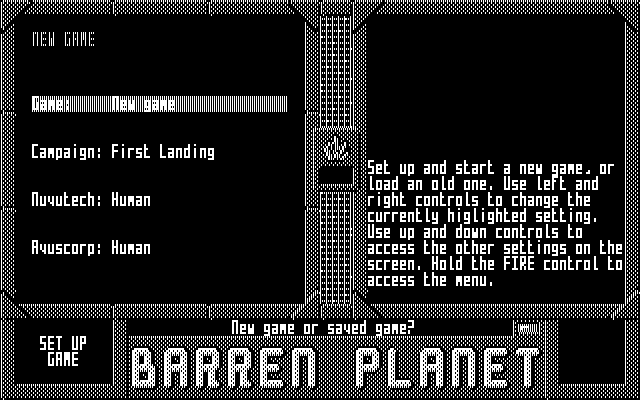
\includegraphics[width=\textwidth]{new-game}
  \caption{The Set up Game screen.}
\end{figure}

% Basic controls
Before navigating your way around this screen you will need to know the game's controls. The game can be controlled entirely with the cursor movement keys ($\leftarrow$ $\rightarrow$ $\uparrow$ $\downarrow$) and the {\it fire} key, which is your choice of {\it Ctrl}, {\it Space} or {\it Enter}.

% Settings window
On the {\it Set up Game} screen, the $\uparrow$ and $\downarrow$ controls move the higlighted bar that you can see in the top left window, allowing you access to the different settings. The $\leftarrow$ and $\rightarrow$ controls will cycle through the available options for the current setting.

% Bringing up the menu
The {\it fire} control brings up the menu, which will appear in the bottom left window. You need to hold this down while navigating the menu using the $\uparrow$ and $\downarrow$ controls, and release it when the option you want to use is highlighted.

% Common options
Every menu starts with a {\it Cancel menu} option that does nothing; it's there for those occasions when you bring up the menu by mistake. All menus also have an {\it Exit game} option that allows you to quit to DOS at any point. Your current state is saved, including any game in progress, and the program will return to this exact point when you run it again. All menus other than the one on the {\it Set up Game} screen have a {\it New Game} option which saves your current game and brings you to this screen.

% Context Sensitive
The program tries to be intelligent when it brings up the menu, highlighting the choice that it thinks you will want at this point. This allows you to choose the most common option by just tapping {\it fire}. On the {\it Set up Game} screen the default option is {\it Start Game}, so on this screen you can just tap {\it fire} to accept the options shown and start your game.

% Choosing a Side
\section{Choosing a Side}

% yes, there is a choice
\noindent
In a single-player game like the one you are about to start, you can choose to play either side. When you first run {\it Barren Planet}, the sides are set up so that {\it Nuvutech} is played by a human and {\it Avuscorp} is played by the computer.

% controls
If you want to play as {\it Avuscorp} instead, use the controls described already to highlight {\it Avuscorp} and change its option to {\it Human}. Then move up to {\it Nuvutech} and change its option to {\it Computer (Easy)}. For the purposes of this tutorial you can play either side, but make sure that the other one is set to {\it Computer (Easy)}. Note that the controls will make sure that at least one of the players is {\it Human}; computer-vs-computer demonstration games are not supported.

% Nuvutech and Avuscorp
In the {\it First Landing} campaign, both sides are about equal. They have different preferences for unit types, although when you get to building your own units, you are not restricted by their preferences. {\it Nuvutech} briefings tend to be professional and use excessively managerial language, while {\it Avuscorp} briefings have a more informal and lawless flavour to them.

% On to Play
\section {On to Play}

% The Start Game option
\noindent
When you are happy with your choice of corporation to play, start the game by selecting the default {\it Start Game} option from the menu. As mentioned already, just tapping {\it fire} will do this.

% Random order of play
The order of play is random, so you might see the computer play first. If this happens, you just need to wait for the computer to take its turn, and then you will be able to take yours as described here.

% The briefing screen
At the start of your first turn, you will see the {\it Mission Briefing} screen. In the top left window a map will appear. The battlefield is bigger than this window; you can use the movement controls to scroll around it and examine the terrain and the initial deployment of the units. In the top right is the briefing text. You are advised to read through it, at least on your first playthrough, as it tells you the objective of the forthcoming battle---which at least for the initial battle is not simply to destroy all enemy units.

% The Mission Briefing screen image
\begin{figure}[h]
  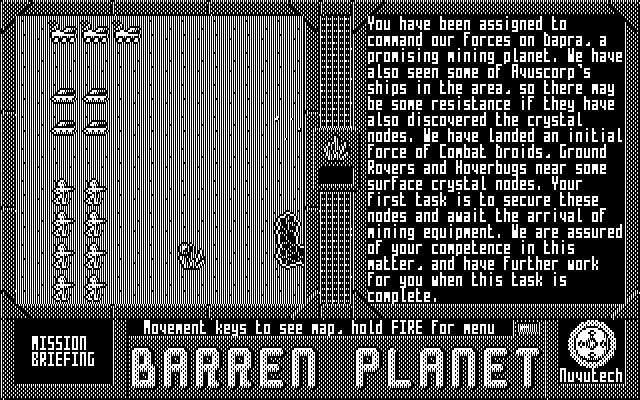
\includegraphics[width=\textwidth]{mission-briefing}
  \caption{The Mission Briefing screen.}
\end{figure}

% Starting Play
When you've taken in all that the {\it Mission Briefing} screen has to tell you, tap {\it fire} to bring up the menu and select the default option, which is {\it Proceed}. This will take you to the {\it Player Turn} screen, where you can start to give orders to your forces.
